% IEEE single-panel figure snippets.
% Use figure* for wide diagrams and qualitative examples; otherwise figure is usually enough.

\begin{figure*}[t]
  \centering
  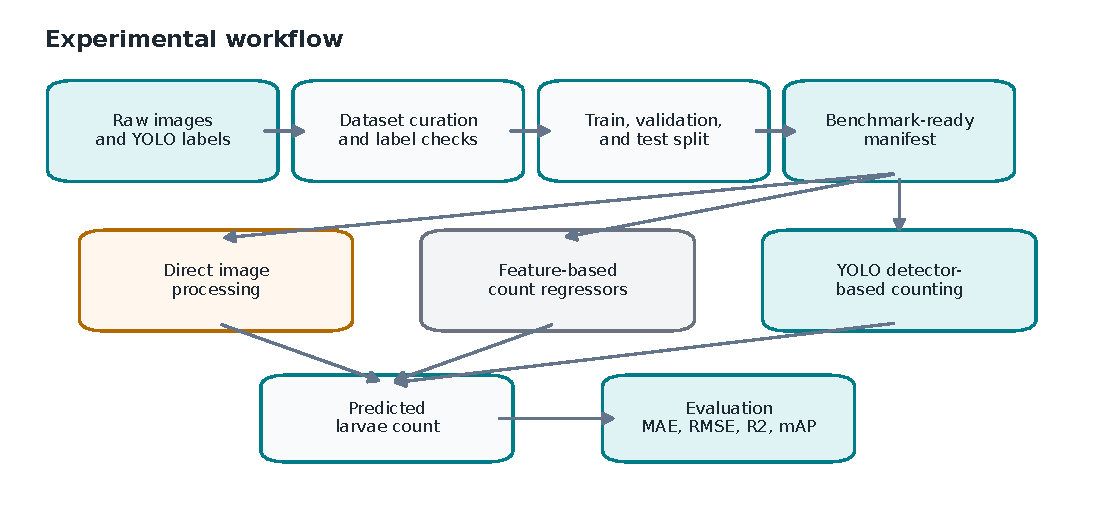
\includegraphics[width=\textwidth]{reports/paper_q4_prep/ieee_figures_split/fig01_methodology_flowchart.pdf}
  \caption{Methodology flowchart.}
  \label{fig:fig01:methodology:flowchart}
\end{figure*}

\begin{figure}[t]
  \centering
  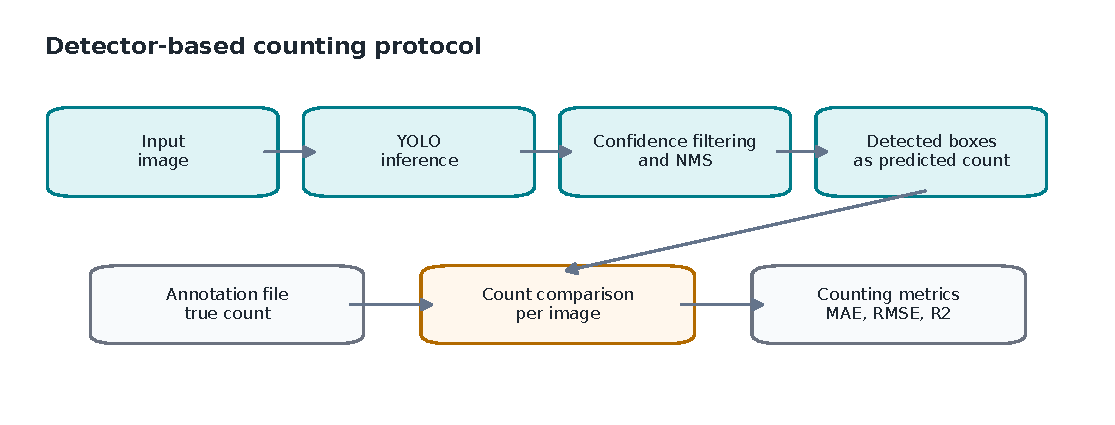
\includegraphics[width=\columnwidth]{reports/paper_q4_prep/ieee_figures_split/fig02_detector_counting_pipeline.pdf}
  \caption{Detector counting pipeline.}
  \label{fig:fig02:detector:counting:pipeline}
\end{figure}

\begin{figure}[t]
  \centering
  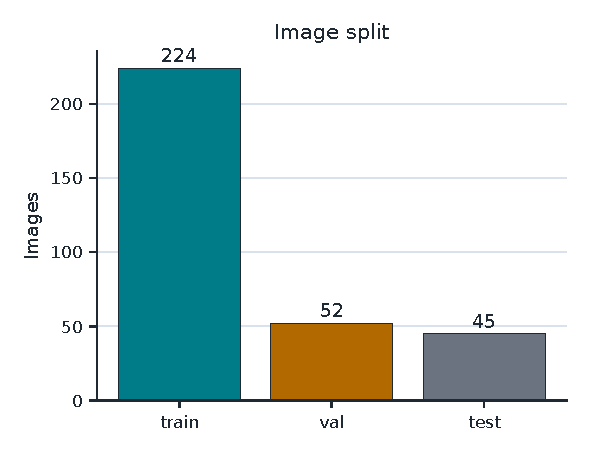
\includegraphics[width=\columnwidth]{reports/paper_q4_prep/ieee_figures_split/fig03_dataset_image_split.pdf}
  \caption{Dataset image split.}
  \label{fig:fig03:dataset:image:split}
\end{figure}

\begin{figure}[t]
  \centering
  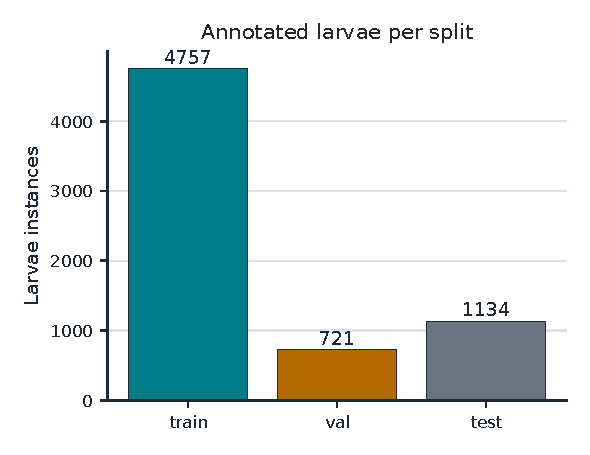
\includegraphics[width=\columnwidth]{reports/paper_q4_prep/ieee_figures_split/fig04_dataset_instance_split.pdf}
  \caption{Dataset instance split.}
  \label{fig:fig04:dataset:instance:split}
\end{figure}

\begin{figure}[t]
  \centering
  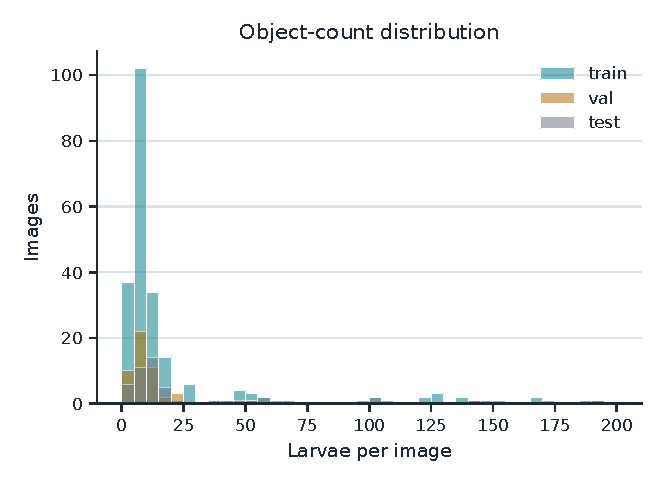
\includegraphics[width=\columnwidth]{reports/paper_q4_prep/ieee_figures_split/fig05_dataset_count_distribution.pdf}
  \caption{Dataset count distribution.}
  \label{fig:fig05:dataset:count:distribution}
\end{figure}

\begin{figure}[t]
  \centering
  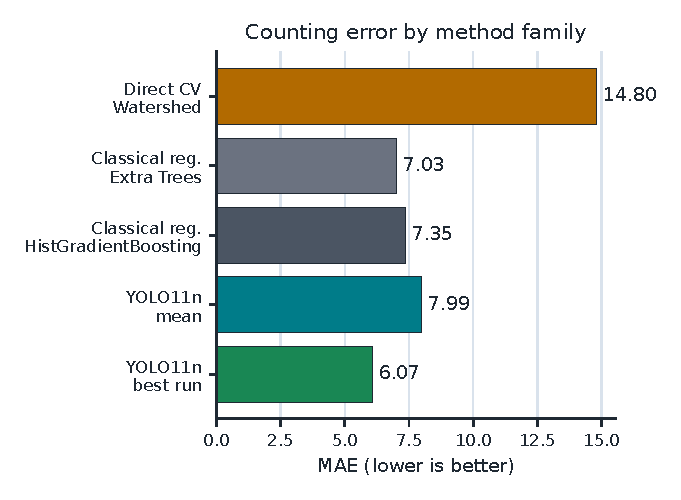
\includegraphics[width=\columnwidth]{reports/paper_q4_prep/ieee_figures_split/fig06_method_family_mae.pdf}
  \caption{Method family mae.}
  \label{fig:fig06:method:family:mae}
\end{figure}

\begin{figure}[t]
  \centering
  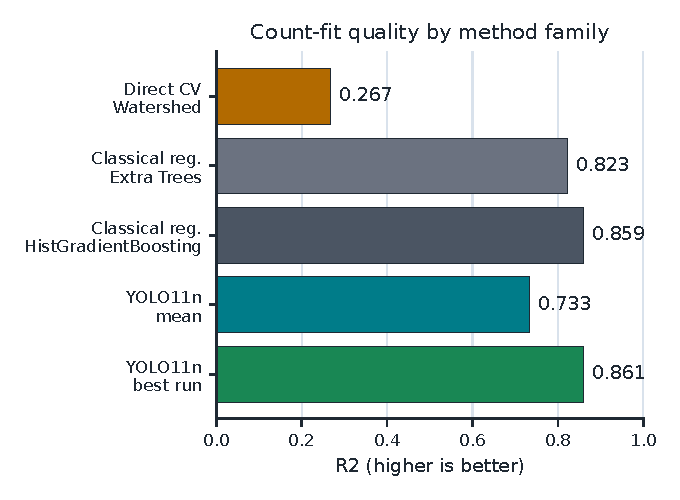
\includegraphics[width=\columnwidth]{reports/paper_q4_prep/ieee_figures_split/fig07_method_family_r2.pdf}
  \caption{Method family r2.}
  \label{fig:fig07:method:family:r2}
\end{figure}

\begin{figure}[t]
  \centering
  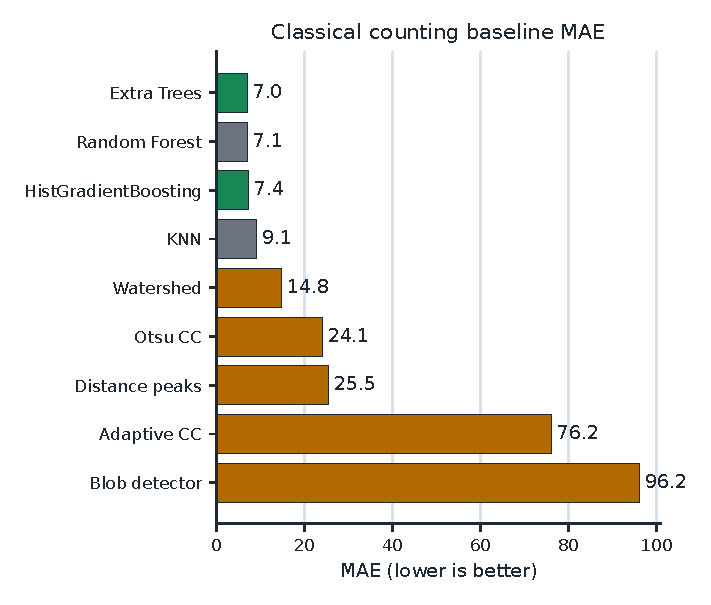
\includegraphics[width=\columnwidth]{reports/paper_q4_prep/ieee_figures_split/fig08_classical_baseline_mae.pdf}
  \caption{Classical baseline mae.}
  \label{fig:fig08:classical:baseline:mae}
\end{figure}

\begin{figure}[t]
  \centering
  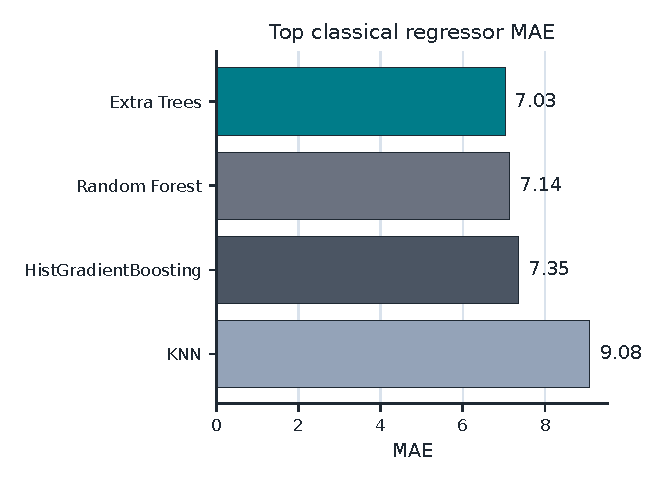
\includegraphics[width=\columnwidth]{reports/paper_q4_prep/ieee_figures_split/fig09_top_classical_mae.pdf}
  \caption{Top classical mae.}
  \label{fig:fig09:top:classical:mae}
\end{figure}

\begin{figure}[t]
  \centering
  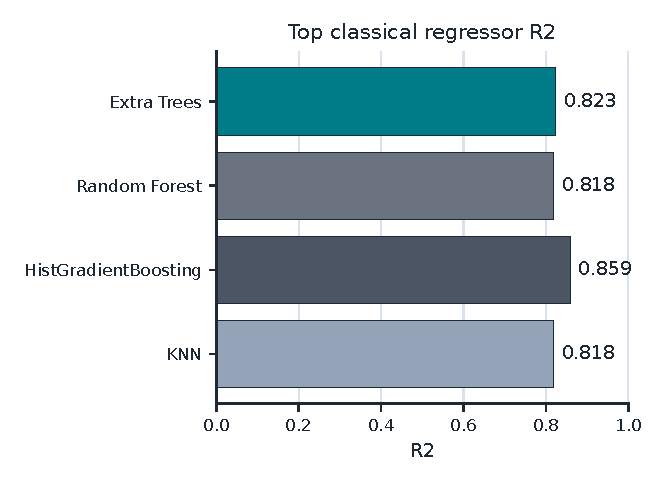
\includegraphics[width=\columnwidth]{reports/paper_q4_prep/ieee_figures_split/fig10_top_classical_r2.pdf}
  \caption{Top classical r2.}
  \label{fig:fig10:top:classical:r2}
\end{figure}

\begin{figure}[t]
  \centering
  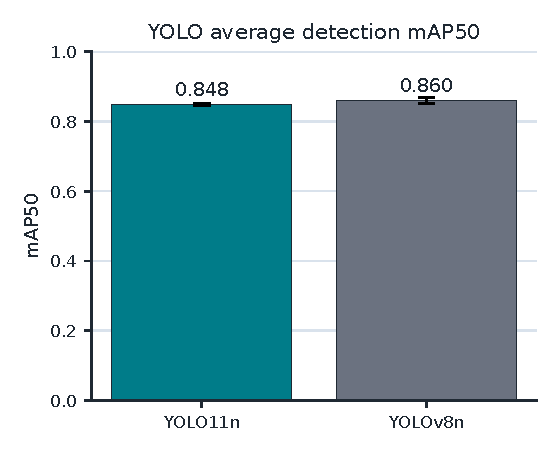
\includegraphics[width=\columnwidth]{reports/paper_q4_prep/ieee_figures_split/fig11_yolo_map50.pdf}
  \caption{Yolo map50.}
  \label{fig:fig11:yolo:map50}
\end{figure}

\begin{figure}[t]
  \centering
  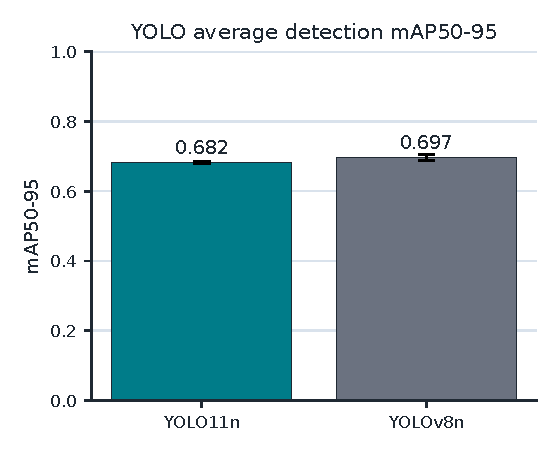
\includegraphics[width=\columnwidth]{reports/paper_q4_prep/ieee_figures_split/fig12_yolo_map50_95.pdf}
  \caption{Yolo map50 95.}
  \label{fig:fig12:yolo:map50:95}
\end{figure}

\begin{figure}[t]
  \centering
  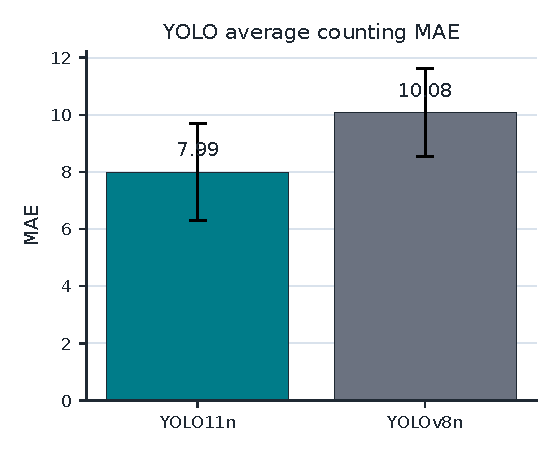
\includegraphics[width=\columnwidth]{reports/paper_q4_prep/ieee_figures_split/fig13_yolo_count_mae.pdf}
  \caption{Yolo count mae.}
  \label{fig:fig13:yolo:count:mae}
\end{figure}

\begin{figure}[t]
  \centering
  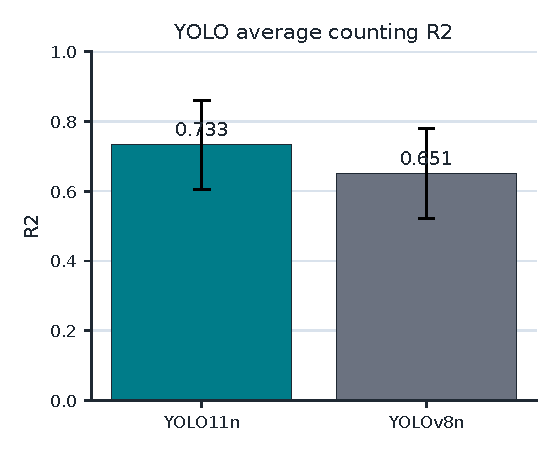
\includegraphics[width=\columnwidth]{reports/paper_q4_prep/ieee_figures_split/fig14_yolo_count_r2.pdf}
  \caption{Yolo count r2.}
  \label{fig:fig14:yolo:count:r2}
\end{figure}

\begin{figure}[t]
  \centering
  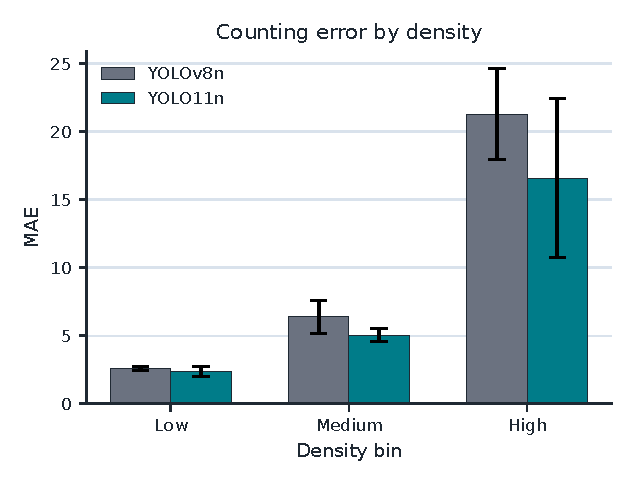
\includegraphics[width=\columnwidth]{reports/paper_q4_prep/ieee_figures_split/fig15_density_mae.pdf}
  \caption{Density mae.}
  \label{fig:fig15:density:mae}
\end{figure}

\begin{figure}[t]
  \centering
  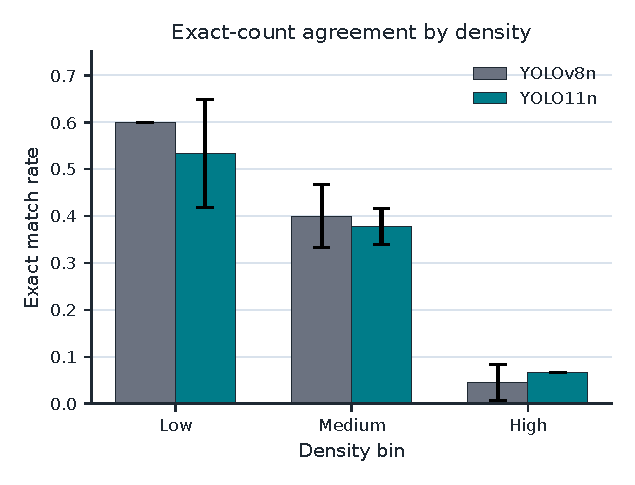
\includegraphics[width=\columnwidth]{reports/paper_q4_prep/ieee_figures_split/fig16_density_exact_match.pdf}
  \caption{Density exact match.}
  \label{fig:fig16:density:exact:match}
\end{figure}

\begin{figure}[t]
  \centering
  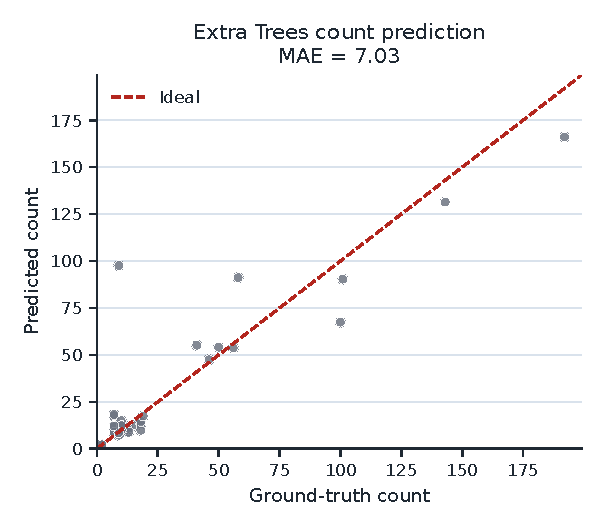
\includegraphics[width=\columnwidth]{reports/paper_q4_prep/ieee_figures_split/fig17_scatter_extra_trees.pdf}
  \caption{Scatter extra trees.}
  \label{fig:fig17:scatter:extra:trees}
\end{figure}

\begin{figure}[t]
  \centering
  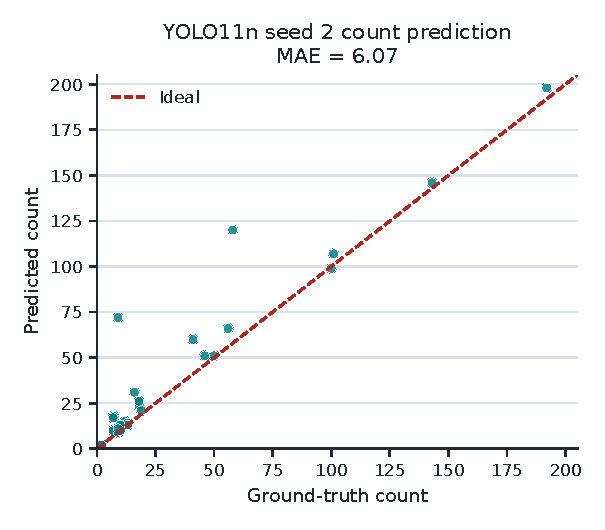
\includegraphics[width=\columnwidth]{reports/paper_q4_prep/ieee_figures_split/fig18_scatter_yolo11n_seed2.pdf}
  \caption{Scatter yolo11n seed2.}
  \label{fig:fig18:scatter:yolo11n:seed2}
\end{figure}

\begin{figure}[t]
  \centering
  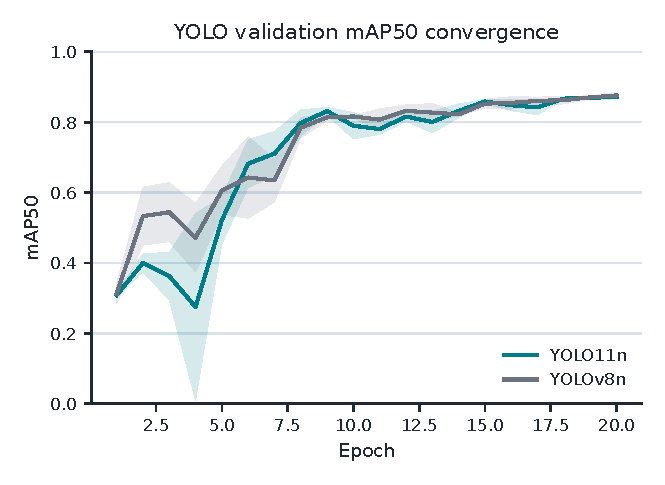
\includegraphics[width=\columnwidth]{reports/paper_q4_prep/ieee_figures_split/fig19_training_map50.pdf}
  \caption{Training map50.}
  \label{fig:fig19:training:map50}
\end{figure}

\begin{figure}[t]
  \centering
  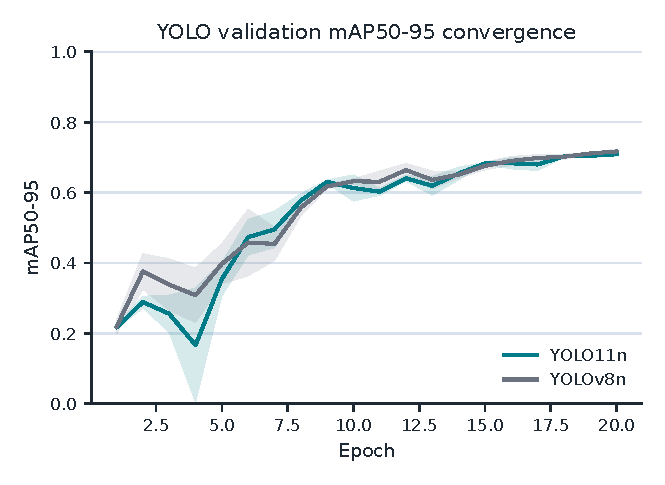
\includegraphics[width=\columnwidth]{reports/paper_q4_prep/ieee_figures_split/fig20_training_map50_95.pdf}
  \caption{Training map50 95.}
  \label{fig:fig20:training:map50:95}
\end{figure}

\begin{figure*}[t]
  \centering
  \includegraphics[width=\textwidth]{reports/paper_q4_prep/ieee_figures_split/fig21_qualitative_success_failure_examples.pdf}
  \caption{Qualitative success failure examples.}
  \label{fig:fig21:qualitative:success:failure:examples}
\end{figure*}
